\documentclass[a4paper,12pt,french]{article}
\usepackage[utf8]{inputenc}
\usepackage[french]{babel}
\usepackage{csquotes}
\usepackage[T1]{fontenc}
\usepackage{geometry}
\usepackage{graphicx}
\usepackage[ruled,french]{algorithm2e}
\usepackage{amsmath}
\usepackage{amssymb}
\usepackage{amsthm}
\usepackage{fancyhdr}
\usepackage{hyperref}
\usepackage{float}
\usepackage{lscape}
\usepackage{array}
\usepackage[normalem]{ulem} % https://github.com/plk/biblatex/issues/193
% \usepackage{import}
\usepackage{afterpage}
\usepackage{xcolor}
\usepackage{graphicx}
\usepackage{tikz}
\graphicspath{{images/}}
\usepackage{listings}
\usepackage{longtable}
\usepackage[nottoc]{tocbibind}
\usepackage[backend=biber,sorting=none]{biblatex}
\usepackage{pdfpages}

\geometry{a4paper,width=160mm,top=20mm,bottom=20mm,bindingoffset=6mm}

\renewcommand{\thetable}{\Roman{table}}
\renewcommand{\headrule}{
    \vspace{-15pt}
    \hrulefill
    \raisebox{-0pt}{
        \scalebox{0.3}{\begin{tikzpicture}
    % Coordinates
    \coordinate (A) at (2.5,0.5);
    \coordinate (B) at (2.2,1.4);
    \coordinate (C) at (1.5,0.5);
    \coordinate (D) at (0.5,0.5);
    \coordinate (E) at (1.0,1.4);
    \coordinate (F) at (2,2);
    \coordinate (G) at (1.7,2);

    % \tikz \draw[thick,rounded corners=8pt]
    %   (0,0) -- (0,2) -- (1,3.25) -- (2,2) -- (2,0) -- (0,2) -- (2,2) -- (0,0) -- (2,0);
    
    \draw[very thick,rounded corners=0pt]
      (A) -- (B) -- (C) -- (D) -- (E) -- (B) -- (F) -- (G);

    \draw[very thick] (A) circle (0.5);
    \draw[very thick] (D) circle (0.5);
    \draw[very thick] (A) circle (0.4);
    \draw[very thick] (D) circle (0.4);
    \filldraw [very thick] (A) circle (0.05);
    \filldraw [very thick] (D) circle (0.05);
    \draw[very thick] (C) circle (0.15);

    \coordinate (H) at (1.8,0.2);
    \coordinate (I) at (1.63,0.2);
    \coordinate (J) at (0.8,1.8);
    \coordinate (K) at (0.6,1.8);
    
    \draw[very thick,rounded corners=0pt]
      (H) -- (I) -- (J) -- (K);

\end{tikzpicture}
}
    }
    \hrulefill
}

\setlength{\headheight}{24pt}
\pagestyle{fancy}
\fancyhf{}
% \fancyhead[LE]{\nouppercase{\rightmark\hfill\leftmark}}
% \fancyhead[RO]{\nouppercase{\leftmark\hfill\rightmark}}
% \fancyfoot[LE,RO]{\hfill\thepage\hfill}

\fancyhead[L]{INSA Rouen}
\fancyhead[R]{LIFAT}

%lien
\hypersetup{
    colorlinks=true,
    linkcolor=black,
    filecolor=magenta,     
    urlcolor=blue,
    citecolor=blue,
}

\addbibresource{bib.bib} % this file should be created
\frenchspacing
\allowdisplaybreaks

\begin{document}
% Meta content 
\title{Optimisation des réseaux cyclables pour l'équité d'accès.}
\author{Lucas JOUBIN}
\date{\today}

\makeatletter
\let\thetitle\@title
\let\theauthor\@author
\let\thedate\@date
\makeatother

\begin{titlepage}
	\begin{minipage}{0.5\textwidth}
		\begin{flushleft} 
\includegraphics[width=0.5\textwidth]{images/LOGOLIFAT700x400.png}
			\end{flushleft}
			\end{minipage}
			\begin{minipage}{0.5\textwidth}
            
			\begin{flushright} 
\includegraphics[width=0.65\textwidth]{images/logo_insa.png}
		\end{flushright}
        
	\end{minipage}\\[.5 cm]
	    
    \begin{center}
        {\Large INSA Rouen Normandie}\\[1. cm]
        \textsc{\LARGE Rapport de stage ingénieur}\\
        \textsc{\Large Recherche opérationnelle}
    \\[1. cm]
    \large effectué au Laboratoire d'Informatique Fondamentale et Appliquée de Tours (LIFAT) \\[.5 cm]
    03 mars 2025 - 25 juillet 2025, 21 semaines.\\[1 cm]
	\rule{\linewidth}{0.2 mm} \\[1 cm]
	{ \huge \bfseries \thetitle}\\[.7 cm]
	\rule{\linewidth}{0.2 mm} \\[1 cm]
    	{\Large Lucas JOUBIN}\\[.2 cm]
    	{\large Génie Mathématique}\\[1 cm]
    \end{center}
	\begin{minipage}{0.5\textwidth}
		\begin{flushleft} \large
		  \textbf{Laboratoire LIFAT}\\
		  64 avenue Jean Portalis\\
            37200 Tours\\
		\end{flushleft}
	\end{minipage}
	\begin{minipage}{0.5\textwidth}
        \begin{flushright} \large
			\textbf{Tutrice dans l'organisme d'accueil} \\
			Tifenn Rault\\
            Maîtresse de conférences \\
            \textbf{Enseignant référent} \\
			Arnaud Knippel\\
		\end{flushright}
	\end{minipage}\\[2 cm]
	\begin{center} Le \thedate
	\end{center}
\end{titlepage}


\clearpage
% \thispagestyle{empty}
\hfill
\clearpage

\section*{Remerciements}
% Je tiens tout d'abord à remercier Monsieur Arnaud SANDER, fondateur d'UNEEK SARL, qui, en m'accueillant au sein de son entreprise, m'a permi d'avoir une première expérience très enrichissante dans le domaine du développement Web. En étant également mon tuteur de stage, Monsieur Arnaud SANDER m'a fait profiter de sa vision d'ensemble des missions à accomplir, en plus de m'avoir offert un accompagnement solide.

% Je souhaite remercier Madame Isabelle SANDER, chargée de mission Ressources Humaines et RSE, pour sa disponibilité et pour m'avoir fait confiance.

% Je souhaiterais remercier tout particulièrement Monsieur Lionel CHAUVIN, développeur senior, qui m'a épaulé sur les points techniques de mon travail et qui m'a surtout transmis son expertise et sa passion, ainsi que Valentin DEVINEAU, développeur, pour son aide et ses conseils. Je remercie en outre le restant des collaborateurs d'UNEEK.

% Je tiens finalement à remercier l'INSA de Rouen et le département Génie Mathématique, l'accompagnement dont j'ai bénéficié m'a permis de trouver un stage adhérant à mon projet professionnel, et dont la qualité de ma formation m'a permis de contribuer au développement d'une entreprise.

\newpage
\tableofcontents
\newpage

\section{Lexique}

\setlength{\parskip}{1em}

\section{Introduction}
\subsection{Contexte du stage}

TODO revoir continuer 

Dans un contexte de transition écologique, la mobilité douce est de plus en plus mise en avant. Le vélo est un moyen de transport qui permet de réduire les émissions de gaz à effet de serre, mais il est encore peu utilisé dans les villes françaises. Pour encourager son utilisation, il est important de développer des infrastructures cyclables adaptées et accessibles à tous les usagers.

Le vélo est de plus un moyen de transport bénéfique pour la santé, et il est donc important de le rendre accessible à tous les usagers, quel que soit leur niveau d'expérience. Cependant, les infrastructures cyclables sont souvent inadaptées aux besoins des usagers, ce qui peut décourager leur utilisation.

\subsection{Présentation de l'entreprise}

Le Laboratoire d'Informatique Fondamentale et Appliquée de Tours (LIFAT) \cite{lifat} regroupe des chercheurs et enseignants-chercheurs de l'Université de Tours et de l'INSA Centre Val de Loire. En 2025, il compte 47 enseignants-chercheurs (professeurs, maîtres de conférences), 31 doctorants et 10 post-doctorants.

Le laboratoire est donc spécialisé en Sciences des Données, avec des spécialités reconnues dans les domaines de l'Intelligence Artificielle et de l'Optimisation.

Le LIFAT a une expérience en matière de collaborations académiques (au niveau national et international) et de partenariats industriels. Les nombreuses opportunités de transfert technologique (vers le monde social et économique) des recherches menées dans le laboratoire ont donné lieu à la création d'un Centre d'Expertise et de Transfert Universitaire (CETU) au laboratoire appelé ILIAD.

Le laboratoire est actuellement organisé en trois équipes de recherche :

\begin{itemize}
    \item Bases de données et Traitement du langage naturel (BdTln)
    \item Reconnaissance des Formes et Analyse d'Images (RFAI)
    \item Recherche Opérationnelle, Ordonnancement et Transport (ROOT). J'étais rattaché à cette dernière lors de mon stage.
\end{itemize}

L'équipe ROOT est spécialisée dans l'optimisation combinatoire et la modélisation mathématique. Elle développe des méthodes et des outils pour résoudre des problèmes complexes d'optimisation dans divers domaines d'application, tels que les mobilités urbaines, la santé numérique et l'industrie 4.0.

\subsection{Objectifs du stage}

L'objectif de mon travail est donc d'optimiser un réseau cyclable en fonction d'indicateurs d'équités choisis. En fonction d'un budget fixé, comment optimiser l'équité d'un réseau cyclable ?

\section{Développement du problème traité}

\subsection{Qu'entend-on par "réseau cyclable équitable" ?}

\subsubsection{Le concept d'équité}

Définir ce qu'est l'équité est une tâche complexe. En effet, l'équité est un concept subjectif, qui peut être mesurée avec différentes métriques. Qu'est ce qui doit peser le plus ?

Il est possible de voir l'équité sous plusieurs approches : *équité horizontale et verticale*

\subsubsection{L'équité entre les cyclistes}

Nous retrouvons ce problème lorsque nous essayons de définir ce qu'est un réseau cyclable équitable. Un réseau cyclable équitable permettrait à tous les usagers de se déplacer aussi facilement, quel que soit l'endroit où ils habitent, leur âge, leur niveau d'expérience, etc. 

Par exemple, on peut considérer que l'équité est atteinte lorsque tous les usagers ont accès aux mêmes infrastructures, ou lorsque les infrastructures sont adaptées aux besoins de chaque usager.

Pour un réseau cyclable, l'équité horizontale se réfère par exemple à l'égalité d'accès aux infrastructures pour tous les usagers, tandis que l'équité verticale se réfère à l'adaptation des infrastructures aux besoins de chaque usager.



Un travail de réflexion sur qu'est ce que l'équité, qu'est ce qui doit être priorisé et sur quel(s) critère(s) d'équité choisir a été réalisé par Lou-ann Deniau, en stage au département Génie de l'Aménagement et Environnement de Polytech Tours en même temps que moi. En se concertant, nous avons pu définir des critères d'équité pour l'optimisation du réseau cyclable, qui soient à la fois pertinents et réalisables informatiquement, en fonction des données présentes, des données que l'on peut croiser, de ce qui ne soit pas trop dur à programmer.

Il existe plusieurs aspects à prendre en compte pour juger de l'équité d'un réseau cyclable. On peut les regrouper en six catégories : 

% \begin{equation}\label{key}
%    \parbox{1\textwidth}{
%         \begin{itemize}
%         \item Les caractéristiques socio-démographiques
%         \item L'accès à un vélo et à une infrastructure cyclable
%         \item Les infrastructures et la cyclabilité
%         \item L'accès à un stationnement vélo et aux opportunités
%         \item Les motifs du trajet
%         \item La diversité des opportunités de destination
%     \end{itemize}
%    }
% \end{equation}

\begin{itemize} \label{categories_eq}
    \item Les caractéristiques socio-démographiques
    \item L'accès à un vélo et à une infrastructure cyclable
    \item Les infrastructures et la cyclabilité
    \item L'accès à un stationnement vélo et aux opportunités
    \item Les motifs du trajet
    \item La diversité des opportunités de destination
\end{itemize}
Elles sont présentées dans la figure \ref{fig:d1}.

\begin{figure}[h]
    \centering
    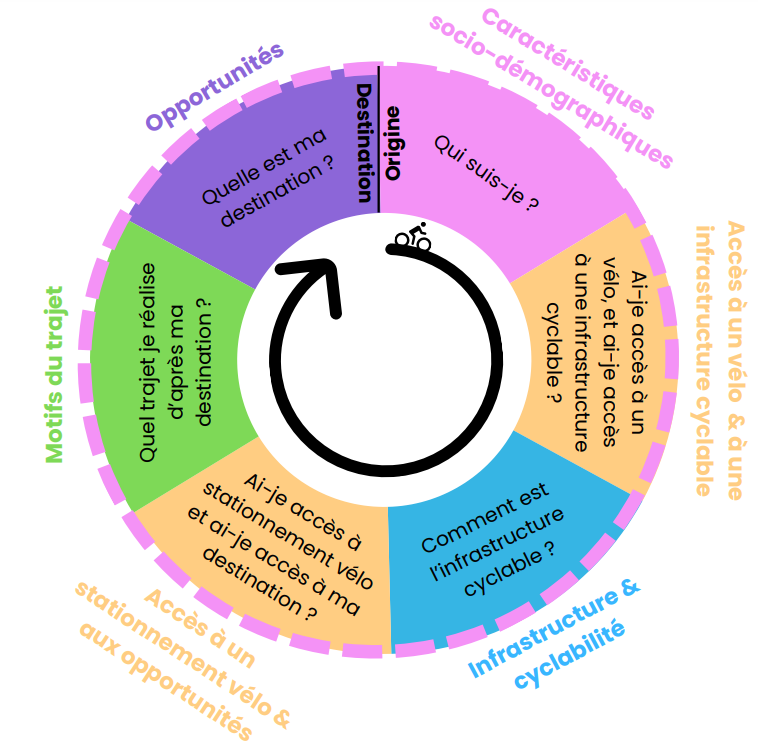
\includegraphics[width=0.5\linewidth]{deniau.png}
    \caption{Déroulé d'un trajet en vélo sous toutes ses dimensions - DENIAU, 2025}
    \label{fig:d1}
\end{figure}

\subsection{Modélisation}

\subsubsection{Routes}

Graphe ayant pour arcs (orientés) les routes (tous les endroits où les vélos ont le droit d'accéder, développer ça) et comme noeuds les intersections entre ces routes. On associe à chaque arc son danger (LTS). 

\subsubsection{Points d'intérêts}

Viennent d'OSM etc développer

\subsubsection{Récupérer les données socio-économiques}

Pour relier le réseau cyclable aux données socio-économiques du territoire, nous utilisons les données Filosofi. On les attache au graphe grâce à un système de noeud délégué.


\subsubsection{Level of Traffic Stress (LTS)}

Le facteur danger est un indicateur de la sécurité des pistes cyclables, calculé en fonction de la distance et du danger associé à chaque segment de voie (arc) Ce calcul est complété
par une classification LTS (Level of Traffic Stress), qui attribue à chaque segment de voie un
niveau de stress allant de 1 à 4, en fonction du profil des cyclistes susceptibles de l'emprunter.

\begin{itemize}
    \item LTS 1 : "Interested but concerned" child (Enfant intéressé mais inquiet)
    \item LTS 2 : "Interested but concerned" adult (Adulte intéressé mais inquiet)
    \item LTS 3 : "Enthused and confident" cyclist (Cycliste enthousiaste et confiant)
    \item LTS 4 : "Strong and fearless" (Assuré et sans peur)
\end{itemize}

LTS 1 et LTS 2 représentent des voies à faible stress (low-stress) qui conviennent aux cyclistes les plus vulnérables, tandis que LTS 3 et LTS 4 indiquent des routes à fort stress (high-stress) où seuls les cyclistes plus expérimentés se sentent à l'aise \cite{kent_karner}.

\begin{table}[h]
\centering
\caption{LTS pour la ville de Tours. Les voies avec un facteur supérieur à 1.75 (ces voies sont par exemple des autoroutes) ont été filtrées.}
\vspace{0.5cm}
\begin{tabular}{|c|c|c|}
\hline
\textbf{Facteur} & \textbf{Count} & \textbf{LTS} \\
\hline
1 & 1905 & LTS 1 (Faible stress) \\
1.15 &3094 &LTS 1 (Faible stress)\\
1.3 &5580 &LTS 2 (Faible stress)\\
1.375& 29017& LTS 2 (Faible stress)\\
1.45 &1901 &LTS 3 (Fort stress)\\
1.75 &66934 &LTS 4 (Fort stress)\\
 \hline 
 \textbf{Total} & \textbf{108431} & \\
 \hline 
 \end{tabular}
\label{table:lts_tours}
\end{table}

La table \ref{table:lts_tours} montre que pour la ville de Tours, sur 108431 arcs, plus de la moitié ont un facteur de danger de 1.75. 

Le facteur LTS de chaque arc est récupéré grâce aux données de Géovélo, une application de navigation pour les cyclistes. En revanche, ces données ne sont pas disponibles en open data, et leur mode de calcul n'est pas précisé. 

Lors de l'optimisation, lorsqu'on améliore des arcs, on met leur LTS à 1 pour calculer les indicateurs d'équité par la suite.

Pour intégrer tous ces aspects à l'optimisation, nous avons considéré les choses suivantes :
\begin{itemize}
    \item Les caractéristiques socio-démographiques sont prises en compte grâce aux carreaux Filosofi. On peut extraire différentes données : il est par exemple possible d'optimiser le réseau seulement pour les enfants de moins de 14 ans, il est aussi possible de faire peser davantage les carreaux où la population a un niveau de vie inférieur à la moyenne, ou encore de faire peser davantage les carreaux où la population est plus âgée.

    \item L'accès à un vélo et à une infrastructure cyclable est pris en compte implicitement par le modèle, qui va chercher à expandre le réseau cyclable pour qu'il soit accessible à un maximum de personnes. 
    % Généralement, le centre ville sera plutôt sécurisé, et les zones périphériques seront moins sécurisées. Les arcs à améliorer se trouvent plutot à l'
    % REVOIR ^si vrai
    
    Il serait possible de prendre ça en compte explicitement, pour que l'optimisation soit encore plus axée sur ce domaine.

    \item Les infrastructures et la cyclabilité sont prises en compte par la classification LTS, qui permet de juger de l'accessibilité d'un réseau cyclable pour un type d'utilisateur en particulier.
    \item L'accès à un stationnement vélo et aux opportunités est pris en compte par la distance maximale qu'un utilisateur est prêt à effectuer (\texttt{dmax}), qui est un paramètre de l'optimisation. Dans la littérature, cette valeur vaut 5 km. On peut aussi utiliser la distance moyenne lors d'un parcours en vélo, qui est de 1,4 km. 
    \item Les motifs du trajet et la diversité des opportunités de destination sont pris en compte par les POI, à la fois par leur nombre et leur catégorie (éducation, commerce, banques...).
\end{itemize}

Tous ces aspects doivent être cohérents entre eux, et il est donc important de les prendre en compte lors de l'optimisation. 

Par exemple, si l'on veut optimiser le réseau cyclable pour les enfants de moins de 14 ans, nous utiliserons aussi un \texttt{dmax} inférieur au cas où l'on optimise le réseau cyclable pour tous les utilisateurs. Les POI conservés seront seulement les écoles, les parcs, etc, mais nous pouvons supprimer les banques et les bureaux. La fréquence de ces POI sera pondérée par la population de chaque carreau INSEE, en faisant peser davantage (ou uniquement) la population des enfants de moins de 14 ans. (juste un exemple pcq pas de programme de ce type)


\subsection{Optimisation}

Nous faisons tout d'abord l'hypothèse suivante : le coût d'une amélioration est proportionnel à la distance de l'arc modifié, le budget peut donc s'exprimer en mètres de route à aménager.

Pour représenter le réseau cyclable (c'est à dire toutes les routes et chemins pouvant être empruntés potentiellement par les cyclistes), nous utilisons un graphe orienté $G(X, A)$ avec $X \ ( \vert X \vert = n)$ l'ensemble des nœuds et $A$ l'ensemble des arcs. A chaque arc est associé son coût en distance, et son danger. 

On dispose de plus d'un ensemble $P$ de POI. Chaque POI p $\in$ P est associé au nœud le plus proche $n_p$ $\in$ $X$ du graphe. 

On dispose également d'un ensemble $Z$ de carreaux couvrant le graphe. Pour chaque zone, on trouve le nœud $n_z$ $\in$ $X$ le plus proche du centre. Pour chaque zone $z$, on dispose d'une liste de POI potentiels, notés $L_z$, représentant les POI potentiellement accessibles depuis $n_z$ en $dmax$ km si l'ensemble du réseau était amélioré, c'est-à-dire si toutes les routes étaient sécurisées. On connaît également la population $w$ vivant dans chaque zone. Enfin, la fonction succ($i$) renvoie les successeurs du nœud $i$ dans le graphe $G$, et la fonction pred($i$) renvoie les prédécesseurs du nœud $i$ dans le graphe $G$.

Nous avons retenu 3 critères d'optimisation différents :

\begin{enumerate}
    \item le nombre de POI totaux atteints, 
    \item le nombre de personnes pouvant atteindre un POI, 
    \item le nombre de catégories différentes de POI atteintes par chaque carreau,
\end{enumerate}

\begin{enumerate}
    \item minimiser le nombre de POI potentiels mais non atteints, 
    \item minimiser le nombre de POI potentiels mais non atteints, 
    \item minimiser le nombre de catégories potentielles mais non atteintes.
\end{enumerate}

Nous conservons les carreaux Filosofi dont la population n'est pas nulle.

Pour optimiser un réseau cyclable, on utilise la programmation linéaire en nombres entiers (PLNE). Le modèle prend en compte différents aspects : TODO

\subsubsection{Modèles exacts}

\subsubsection{Heuristiques}

Pour les heuristiques sur la population et sur le nombre de POI, le schéma est le suivant :

\begin{figure}[H]
    \centering
    \begin{algorithmic}
    \STATE $i\gets 10$
    \IF {$i\geq 5$} 
    \STATE $i\gets i-1$
    \ELSE
    \IF {$i\leq 3$}
        \STATE $i\gets i+2$
    \ENDIF
    \ENDIF 
    \end{algorithmic}
    \caption{algo 1}
\end{figure}



\subsection{2 visibilités différentes}

L'optimisation par CPLEX s'effectue sur deux visibilités différentes : 

\begin{itemize}
    \item La \textbf{visibilité exacte}, où la visibilité d'une tuile comprend toutes les arêtes qui lui sont à une distance inférieure à la distance maximale \texttt{dmax}.

    Etant donné que \texttt{dmax} ne peut pas être dépassé lors de la recherche du résultat optimal, ce modèle donne le même résultat que si tout le graphe était visible, la visibilité est bien exacte. Cette technique permet de rendre CPLEX plus rapide. 

    \item La \textbf{visibilité réduite}, où la visibilité d'un carreau comprend toutes les arêtes qui sont dans un plus court chemin (PCC) d'un nœud délégué jusqu'à un point d'intérêt, tout en respectant la contrainte de distance de la visibilité précédente.

    La visibilité d'un carreau comprend aussi les arêtes se trouvant dans un PCC allant d'un nœud délégué d'un \textit{autre} carreau à un POI, tant que ces arêtes sont à moins de \texttt{dmax} de distance du carreau.
\end{itemize} 

**mettre schéma**


\subsection{Visualisation de l'équité d'un réseau cyclable}

Pour juger de l'équité d'un réseau cyclable pour un type d'utilisateur en particulier, on peut ajouter des malus pour certaines spécificités du réseau. Par exemple, si le réseau comporte beaucoup de discontinuités (c'est à dire des passages dangereux, comme une route à traverser, parsemant une piste cyclable sûre), il n'est pas adapté à des enfants de moins de 14 ans. On peut donc ajouter un malus pour les discontinuités si l'on veut visualiser l'équité d'un réseau cyclable pour des enfants de moins de 14 ans.

Un des aspects les plus importants pour juger de l'équité d'un réseau cyclable est le niveau d'expérience et d'aise des utilisateurs. En revanche, il est difficile de récupérer ce type de données : pas d'études sur la ville de Tours ont été réalisées. Il faudrait en effet avoir des données pour chaque carreau INSEE de la ville.

Une autre chose intéressante à prendre en compte pour calculer l'équité d'un réseau cyclable est le réseau de transports en commun. En effet, si un endroit est mal desservi par les transports en commun, il est d'autant plus nécéssaire d'avoir un réseau cyclable fonctionnel. 
% Cette chose est aussi difficile à prendre en compte, parce qu'elle nécessiterait de croiser des données (ou peut etre pas avec les POI?)




\subsection{Critères d'optimisation}

Les critères d'optimisations vont directement être en lien avec visualisation de l'équité d'un réseau cyclable. En effet, la mesure de l'existant amène à créer un nouveau critère, et la solution trouvée par l'optimisation va être ensuite évaluée en visualisant. revoir paragraphe

\subsection{Résultats}

Les instances étant trop couteuses pour être lancées en local (Processeur Intel(R) Pentium(R) CPU 5405U @ 2.30GHz, 8 Go de mémoire RAM), mes tests ont été effectués sur le Mésocentre de Calcul CaSciModOT \cite{cas}. C'est un centre régional de calcul parallèle de taille intermédiaire entre des stations de travail et les grands centres nationaux (CINES, IDRIS, CCRT). Il permet de fournir à l'ensemble des partenaires de la fédération CaScIModOT une grappe possédant une puissance de calcul hautes performances.

Les calculs sont lancés sur un processeur AMD Epyc 7702 à 2GHz,.

% \resizebox{10cm}{!}{
\begin{table}[h]
\centering
\caption{Résultats pour une instance comprenant 500 noeuds}
\vspace{0.5cm}
\begin{tabular}{|c|c|c|c|c|c|c|c|c|c|c|c|c|c|c|}
% \begin{tabular}{|c c c c c c c c c c c c c c c|}
\hline
% B & dmax & lts & Obj value
% cplex
% exact & Obj value
% cplex PCC
% exact & Obj value
% cplex PCC
% de cplex & Obj value
% heuristique & reached
% POI cplex
% exact & reached
% POI cplex
% PCC & reached
% POI
% heuristique  & time
% cplex
% exact & time
% cplex
% PCC & time
% heuristique & gap obj val
% cplex exact/
% cplex PCC & gap obj val
% cplex PCC/
% heuristique \\
% \hline
1000 & 400 & 1 & 247 & 253 & 253 & 259 & 50.0 & 44.0 & 38.0 & 3523.54 & 0.48 & 0.0 & 0.976 & 0.977 \\
1000 & 500 & 1 &  & 435 & 435 & 443 &  & 46.0 & 38.0 &  & 1.07 & 0.0 &  & 0.982 \\
1000 & 400 & 1.3 & 114 & 125 & 147 & 181 & 183.0 & 172.0 & 130.0 & 770.37 & 0.26 & 0.0 & 0.912 & 0.812 \\
1000 & 400 & 1.44 & 45 & 57 & 79 & 116 & 252.0 & 240.0 & 199.0 & 583.75 & 13.53 & 0.0 & 0.789 & 0.681 \\
2000 & 1000 & 1 &  & 1659 & 1660 & 1701 &  & 95.0 & 53.0 &  & 39.73 & 0.01 &  & 0.976 \\
2000 & 400 & 1 & 212 & 223 & 226 & 244 & 85.0 & 74.0 & 53.0 & 5012.11 & 0.41 & 0.0 & 0.951 & 0.926 \\
2000 & 400 & 1.44 & 19 & 33 & 41 & 94 & 278.0 & 264.0 & 225.0 & 237.8 & 0.33 & 0.0 & 0.576 & 0.436 \\
2000 & 800 & 1.44 &  & 184 & 350 & 637 &  & 1035.0 & 819.0 &  & 3.77 & 0.01 &  & 0.549 \\
 \hline 
 \end{tabular}
\end{table}

L'efficacité est calculée par erreur relative \cite{erreur_relative}.

Des tests ont été effectués avec une heuristique qui remplit le budget au maximum, mais les résultats sont similaires pour la gamme de paramètres utilisée.

*mettre tableau comparaison*

Pour Tours, de plus grandes valeurs des paramètres nécéssitaient plus de 512go de mémoire.

\subsubsection{Comparaison des valeurs trouvées par "accident"}

Lorsqu'on lance CPLEX sur le modèle à visibilité réduite, des POI sont trouvés par "accident" : certains chemins entre un noeud délégué et un POI ne sont pas visibles par le modèle, puisque certaines arêtes sont amputées au modèle. Donc, lorsqu'on recompte manuellement le nombre de POI à présent accessibles, ils sont davantage que la valeur objective retournée par CPLEX. La table \ref{table:lts_tours} montre l'ampleur de ce phénomène pour différentes instances.

Lorsqu'on compare les valeurs objectives de CPLEX pour ces deux visibilités, il faut prendre en compte ce biais.

Voir 2 visibilités différentes

\subsubsection{S'assurer de la cohérence des résultats entre les 2 projets}

J'ai repris deux projets déjà entamés par le LIFAT, Bike Accessibility (optimisation d'un réseau cyclable) et Chemins Equitables (visualisation d'indicateurs d'équités). J'ai ensuite dù faire communiquer ces deux projets. 

Dans les projets Bike Accessibility et Chemins Equitables, certaines étapes étaient effectuées différemment, par exemple compter les POI accessibles, ou encore la reindexation des noeuds. Il était donc important de s'assurer que les résultats trouvés étaient les mêmes entre les deux projets. Sur la figure \ref{fig:nb_poi_compa}, on peut voir une comparaison visuelle des résultats de ces deux projets, pour les POI accessibles.

\begin{figure}[ht]
\centering
    \begin{tabular}{cc}    
        \begin{minipage}[t]{2.5in}
        \centering
        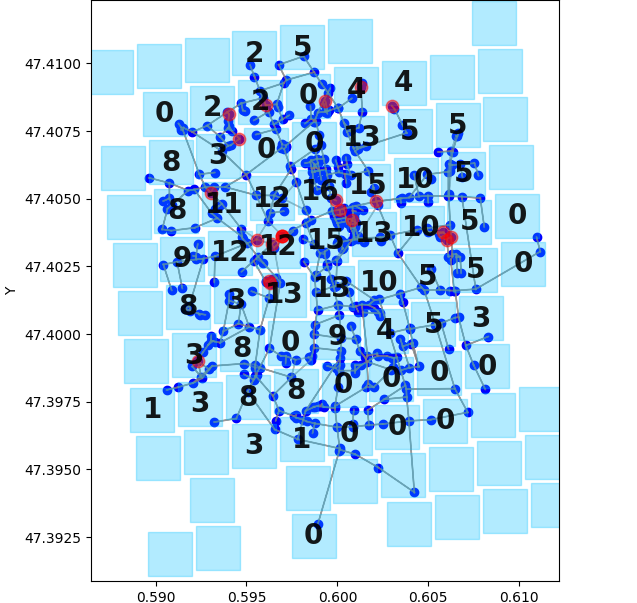
\includegraphics[height=2.5in]{nb_poi_BA.png}
        % \label{fig:task1_l1}
        \end{minipage}
    %%    
        \begin{minipage}[t]{2.5in}
        \centering
        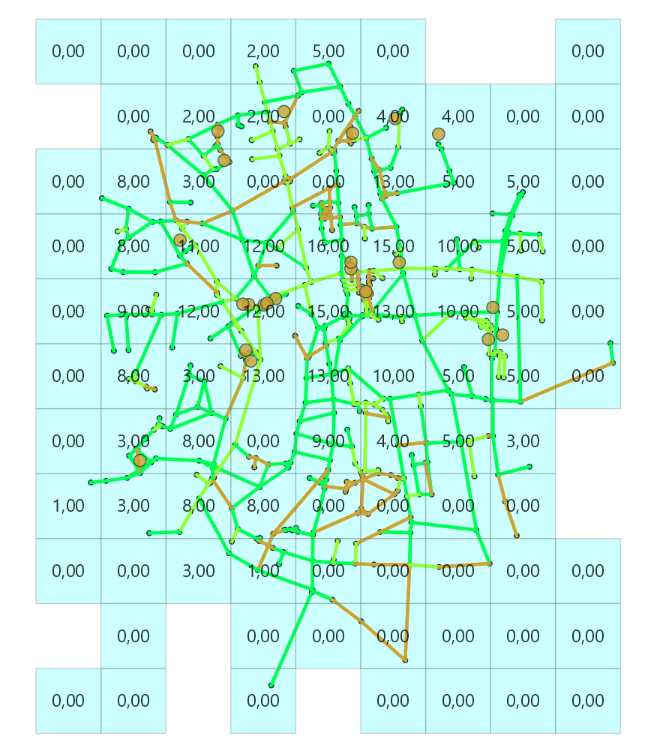
\includegraphics[height=2.5in]{nb_poi_CE.png}
        % \label{fig:task1_cpu}
        \end{minipage}
    \end{tabular}
    \caption{A gauche, le nombre de POI accessibles par carreau INSEE pour le projet Bike Accessibility. A droite, le nombre de POI accessibles par carreau INSEE pour le projet Chemins Equitables. Pour la ville de Fondettes, dans l'agglomération de Tours.}
    \label{fig:nb_poi_compa}
\end{figure}

Voir 2 visibilités différentes


\section{Conclusion}

\subsection{Bilan du stage}

\subsection{Développements ultérieurs}

Il est possible d'ajouter davantage de paramètres pour gagner en réalisme

\subsection{Apport personnel}

Stage pluridisciplinaire, avec des aspects de recherche opérationnelle, de développement informatique et de visualisation de données.

Travail avec des Géographe - cartographe

Travail d'équipe, vulgarisation, expliquer à des personnes qui ne s'y connaissent pas en informatique.

\section{Grille de déroulement du stage}

\begin{longtable}[H]{| m{5cm} | m{10cm} |}
\hline
\textbf{Dates} & \textbf{Tâche effectuée}\\
\hline
\endfirsthead

\hline
\textbf{Dates} & \textbf{Tâche effectuée}\\
\hline
\endhead

\hline
\endfoot

\hline
\endlastfoot

semaine 1 : 03/03 au 07/03 & Prise en main du sujet, du projet Bike Accessibility et de CPLEX. \\
\hline
semaine 2 : 10/03 au 14/03 & Corrections sur la visibilité du modèle CPLEX déjà implémenté.\\
\hline
semaine 3 : 17/03 au 21/03 & Développement d'une première heuristique pour le modèle maximisant le nombre de POI atteints.\\
\hline
semaine 4 : 24/03 au 28/03 & Prise en main de CaSciModOT, lancement de tests, correction de l'heuristique.\\
\hline
semaine 5 : 31/03 au 04/04 & Création de nouvelles instances et de scripts Python pour déboguer.\\
\hline
semaine 6 : 07/04 au 11/04 & Travail avec un critère d'optimisation sur le nombre de personnes impactées, création d'heuristiques pour ce modèle. \\
\hline
semaine 7 : 14/04 au 18/04 & Déboguage du modèle CPLEX.\\
\hline
semaine 8 : 21/04 au 25/04 & Lancement de tests de comparaison entre tous les modèles, création de tables de comparaison.\\
\hline
semaine 9 : 28/04 au 02/05 & Création de tables de résultats et rédaction sur les résultats. \\
\hline
semaine 10 : 05/05 au 09/05 & Prise en main du projet Chemins Equitables. Relancement de l'optimisation avec des instances réelles (quartiers de la métropole de Tours). \\
\hline
semaine 11 : 12/05 au 16/05 & Modification du projet Chemins Equitables pour qu'il fonctionne avec des fichiers provenant du projet Bike Accessibility. \\
\hline
semaine 12 : 19/05 au 23/05 & Production de résultats graphiques. \\
\hline
semaine 13 : 26/05 au 30/05 & Discussion avec des géographes et des cartographes, modifications en conséquent du projet Chemins Equitables. Réflexion sur de nouveaux critères d'optimisation. \\
\hline
semaine 14 : 02/06 au 06/06 & Création de cartes après correction de bugs et production de documentation.\\
\hline
semaine 15 : 09/06 au 13/06 & Développement d'une heuristique favorisant la diversité de POI. \\
\hline
semaine 16 : 16/06 au 20/06 & Développement de PM (performance measures) pour la diversité de POI, création de cartes. \\
\hline
semaine 17 : 23/06 au 27/06 & Déboguage, tests et rédaction sur les résultats. \\
\hline
semaine 18 : 30/06 au 04/07 & Rédaction, programmation d'un modèle CPLEX sur la diversité de POI. \\
\hline
semaine 19 : 07/07 au 11/07 & Déboguage du modèle CPLEX, tentative de générer les jeux de données compatibles avec la visualisation sur Chemins Equitables dans le projet Bike Accessibility directement. \\
\hline
semaine 20 : 14/07 au 18/07 & Rédaction du rapport de stage, écriture de fichiers README. \\
\hline
semaine 21 : 21/07 au 25/07 & Finalisation du rapport de stage, rédaction d'un document livrable pour les cartographes. \\
\end{longtable}

\newpage
%add bibliography to tablecontent
\printbibliography[
heading=bibintoc,
title={Bibliographie}
]

\newpage
\section*{Annexes}

\subsection*{Modèle PLNE}
\subsection*{Integer Linear Programming Model}\label{annexe:modeleexact}

Given a graph describing the network, costs representing the cost of the roads with and without improvements, a set of zones and their associated population, a set of POI, the model computes the roads to improve within a given budget with the objective to increase the weighted number of POI reachable by the zones within 5 km. Here we consider that the cost of an improvement is proportional to the distance of the arc that is modified. 

%\subsection{Input data (parameters)}

\textbf{Parameters:} The road network is represented by an oriented graph $G(X,A$) with $X$ ($|X|=n$) the set of nodes, and $A$ the set of arcs. Each arc is associated with two costs : $c_{ij}^1$ (resp. $\overline{c_{ij}}^1$ ) is the distance cost of arc $(i,j)$ before (resp. after) improvements. We are given a set $\mathcal{P}$ of POI. Each POI $p \in \mathcal{P}$ is associated to the closest node $n_p \in X$ in the graph. We are also given a set $\mathcal{Z}$ of zones covering the graph, and for each zone we have the node $n_z \in X$ that is closest to the center of the zone. For each zone $z$ we have a list of potential POI, denoted $\mathcal{L}_z$, representing the POI potentially reachable from $n_z$ in 5 km if all the network were improved, i.e if all roads were secure. We also have the population $w_z$ living in each zone. Lastly, function $succ(i)$ returns the successors of node $i$ in graph $G$, and $pred(i)$ returns the predecessors of node $i$ in graph $G$.
 \\

%\textbf{Variables:} We use the following variables :
%\begin{itemize}
%\item $y_{ij}^k$ : $y_{ij}^k = 1$ if arc $(i,j) \in A$ is part of the path $k$ and the arc $(i,j)$ is not modified, $0$ otherwise.
%\item $\overline{y_{ij}}^k$ :  $\overline{y_{ij}}^k = 1 $ if arc $(i,j) \in A$ is part of the path $k$ and the arc $(i,j)$ is modified, $0$ otherwise. 
%\item $\sigma_{ij}$ is equal to 1 if arc $(i,j)$ is not modified, 0 otherwise. When this variable is equal to one, $(i,j)$ must be not modified for all paths going through it.
%\item $\overline{\sigma_{ij}}$ is equal to 1 if arc $(i,j)$ is modified, 0 otherwise. When this variable is equal to one, $(i,j)$ must be modified for all paths going through it.
%\item $\delta_{ij}^k$ is equal to 1 if arc $(i,j)$ is in path $k$ (modified or not).
%\end{itemize}

\textbf{Variables:} The main decision variables are the variables $\overline{\sigma_{ij}}$, which is equal to 1 if arc $(i,j)$ is modified, 0 otherwise. When this variable is equal to one, $(i,j)$ must be modified for all paths going through it. Then, we have variables to model the routing from the center of each zone $n_z$ to its potential reachable POI $p \in \mathcal{L}_z$ : ${\delta_{ij}}_z^p$ is equal to 1 if arc $(i,j)$ is in path from $n_z$ to $n_p$ (modified or not). Finally, to compute the cost of each path, we need the two following variables :
\begin{itemize}
\item ${y_{ij}}_z^p$ : ${y_{ij}}_z^p = 1$ if arc $(i,j) \in A$ is part of the path from $n_z$ to $n_p$ and the arc $(i,j)$ is not modified, $0$ otherwise.
\item $\overline{{y_{ij}}_z^p}$ :  $\overline{{y_{ij}}_z^p} = 1 $ if arc $(i,j) \in A$ is part of the path from $n_z$ to $n_p$  and the arc $(i,j)$ is modified, $0$ otherwise. 
\end{itemize}

We also have the binary variables $\overline{PPOI_z^p}$, which is equal to 1 if the the POI $p$ is NOT reachable in less than 5 km by $n_z$, and variables $I_z$ that count the number of POI not reachable by zone $n_z$ among its potentially reachable POI.

%\subsection{Constraints}
\begin{equation}\label{eq:obj}
Minimize \sum_{z \in \mathcal{Z} } w_z I_z 
\end{equation}

\begin{equation}\label{eq:consIz}
I_z = \sum_{p \in \mathcal{L}_z} \overline{PPOI_z^p}, \forall z \in \mathcal{Z}
\end{equation}

\begin{equation}\label{eq:cons1}
{y_{ij}}_z^p + \overline{{y_{ij}}_z^p} \leq 1,  \forall z \in \mathcal{Z}, \forall p \in \mathcal{L}_z, \forall (i,j) \in A 
\end{equation} 

\begin{equation}\label{eq:cons2}
\overline{\sigma_{ij}} \geq \overline{{y_{ij}}_z^p},  \forall z \in \mathcal{Z}, \forall p \in \mathcal{L}_z, \forall (i,j) \in A 
\end{equation}
\begin{equation}
 1-\overline{\sigma_{ij}} \geq {y_{ij}}_z^p,  \forall z \in \mathcal{Z}, \forall p \in \mathcal{L}_z, \forall (i,j) \in A 
\end{equation}

\begin{equation}\label{eq:path1}
{\delta_{ij}}_z^p = {y_{ij}}_z^p + \overline{{y_{ij}}_z^p},  \forall z \in \mathcal{Z}, \forall p \in \mathcal{L}_z, \forall (i,j) \in A 
\end{equation}

\begin{equation}\label{eq:path2}
\sum_{j \in succ(n_z)} {\delta_{n_z,j}}_z^p =1,  \forall z \in \mathcal{Z}, \forall p \in \mathcal{L}_z 
\end{equation}
\begin{equation}
\sum_{j \in pred(n_p)} {\delta_{j, n_p}}_z^p =1,  \forall z \in \mathcal{Z}, \forall p \in \mathcal{L}_z 
\end{equation}

\begin{equation}\label{eq:path2bis}
\sum_{j \in pred(n_z)} {\delta_{j,n_z}}_z^p =0,  \forall z \in \mathcal{Z}, \forall p \in \mathcal{L}_z 
\end{equation}
\begin{equation}
\sum_{j \in succ(n_p)} {\delta_{n_p,j}}_z^p =0,  \forall z \in \mathcal{Z}, \forall p \in \mathcal{L}_z 
\end{equation}


\begin{equation}\label{eq:path4}
\sum_{i \in pred(j)} {\delta_{i,j}}_z^p = \sum_{l \in succ(j)} {\delta_{j,l}}_z^p  ,   \forall z \in \mathcal{Z}, \forall p \in \mathcal{L}_z , \forall j \in N\backslash \{n_z, n_p\}
\end{equation}
\begin{equation}\label{eq:path5}
\sum_{i \in pred(j)} {\delta_{i,j}}_z^p \leq 1,  \forall z \in \mathcal{Z}, \forall p \in \mathcal{L}_z, \forall j \in N
\end{equation}
\begin{equation}
\sum_{l \in succ(j)} {\delta_{j,l}}_z^p \leq 1,  \forall z \in \mathcal{Z}, \forall p \in \mathcal{L}_z, \forall j \in N
\end{equation}

\begin{equation}\label{eq:limit1}
\sum_{(i,j)\in A} \overline{\sigma_{ij}} c_{ij}^1  \leq B
\end{equation}

\begin{equation}\label{eq:pathcost}
\begin{aligned}
D_z^p = & \sum_{(i,j) \in A} {y_{ij}}_z^p c^1_{ij} 
 + \sum_{(i,j) \in A}  \overline{{y_{ij}}_z^p}  \overline{c_{ij}}^1 , \forall z \in \mathcal{Z}, p \in \mathcal{L}_z \\
\end{aligned}
\end{equation}

\begin{equation}\label{eq:consdistPoi1}
    \overline{PPOI_z^p} \leq \frac{D_z^p}{5}, \forall z \in \mathcal{Z}, p \in \mathcal{L}_z 
\end{equation}

\begin{equation}\label{eq:consdistPoi2}
    \overline{PPOI_z^p} \geq \frac{-(5-D_z^p)}{BigM}, \forall z \in \mathcal{Z}, p \in \mathcal{L}_z 
\end{equation}

%% --------------------------------
Constraints (\ref{eq:consIz}) count the number of POI not reachable by each zone in the modified graph. (\ref{eq:cons1}) and (\ref{eq:cons2}) ensure consistency of $y$ and $\overline{y}$ variables. These constraints ensure that if an arc is modified, it is modified for all paths passing by this arc. Alternatively, if an arc is not modified, it is not modified in other paths. Notice that (\ref{eq:cons1})  is not mandatory due to (\ref{eq:cons2}) formulation.  (\ref{eq:path1}) to (\ref{eq:path5}) guarantee the consistency of the calculated paths between zones center and reachable POI.  (\ref{eq:limit1}) limit the total length of modified arcs with an upper bound B. (\ref{eq:pathcost}) represent the  cost of a path from $n_z$ to $n_p$: this cost takes into consideration whether the arcs are modified or not. It is equal to the distance if all arcs of the path are secure, to infinity otherwise. (\ref{eq:consdistPoi1}) and (\ref{eq:consdistPoi2}) check weather the POI $p$ is reachable in less than 5 km from $n_z$ via secure roads. Finally, the objective function \ref{eq:obj} minimizes the weighted sum of POI not reachable within 5 km.

\subsection*{Extension : considering the diversity of POI.}

In this section, we want to consider the diversity of the POI in the optimization process. Therefore, we adapt the previous model as follows. We now assume that each POI is associated to a category $c \in \mathcal{C}$ (exactly one).

\textbf{Parameters :} $POI^p_c$ is an input data and is equal to one if the POI $p$ is of category $c$. We also denote by $\#POI^z_c$ the number of POI of category $c$ that would be reachable by zone $z$ if all the network were secured.

\textbf{Variables :} We introduce a new variable denoted $cat^z_c$ which is equal to 1 if there exists a path in the modified graph from zone $z$ to at least one POI of category $c$. This variable is introduced in the model thanks to this new constraint:

\begin{equation}
cat^z_c \leq \frac{\sum_{p \in \mathcal{L}_z} \left( POI^p_c \cdot (1 - PPOI^p_z) \right)}{\#POI^z_c}, \quad \forall z \in \mathcal{Z},\ c \in \mathcal{C}
\tag{18}
\end{equation}

The objective function can be modified to account for both the diversity of the reachable POI and the population of the tiles:

\begin{equation}
Maximize \sum_{z \in \mathcal{Z}} \sum_{c \in \mathcal{C}} cat^z_c \cdot w_z
\tag{19}
\end{equation}


\end{document}